\documentclass[11pt]{article}

\usepackage[letterpaper,margin=1in]{geometry}
\usepackage[T1]{fontenc}
\usepackage{lmodern}
\usepackage{graphicx}
\usepackage{booktabs}
\usepackage{caption}
\usepackage{subcaption}
\usepackage{tikz}
\usetikzlibrary{arrows.meta,positioning,calc}
\usepackage[round,authoryear]{natbib}
\usepackage{hyperref}
\usepackage{xcolor}
\usepackage{setspace}
\usepackage{titlesec}

\hypersetup{
  colorlinks=true,
  linkcolor=black,
  urlcolor=blue,
  citecolor=black
}

\onehalfspacing
\setcounter{secnumdepth}{0}

\titleformat{\section}{\large\bfseries}{}{0em}{}
\titleformat{\subsection}{\normalsize\bfseries}{}{0em}{}
\titlespacing*{\section}{0pt}{1.2em}{0.6em}

\title{Severed Accessibility and Urban Resilience:\\A multi-scalar analysis of flood risk in Chennai}
\author{Daniela Res\'endiz Garc\'ia\\
\small BARC0026: Analytical Design Research Project Coursework\\
\small MSc in Space Syntax: Architecture and Cities\\
\small The Bartlett School of Architecture, University College of London\\
\small Supervisor: Prof.\ Alan Penn}
\date{}

\begin{document}
\maketitle

\begin{abstract}
Flooding is a rapidly intensifying urban challenge, disrupting essential services and exposing structural inequalities across cities worldwide. While existing frameworks address either ecological resilience or spatial configuration, few capture how flood events dynamically alter accessibility---disconnecting populations from shelters, services, or safe mobility routes.

This study introduces a spatial methodology that models accessibility loss under extreme flood conditions, integrating a 100-year return period scenario with network-based spatial analysis. Applied to Chennai, the approach overlays flood impact on road networks, land use, and infrastructure to assess where functional accessibility collapses. A clustering analysis further identifies priority zones for safe shelter allocation and evacuation planning.

Results show that accessibility degradation is spatially uneven. Compact urban forms retain greater connectivity under stress, while dispersed or fragmented areas become structurally isolated. Key corridors and intervention areas are mapped both at local and metropolitan scales, offering actionable entry points for adaptive planning.

The method reframes resilience not as physical resistance to flooding, but as the preservation of spatial connection under disruption. It is transferable to diverse urban contexts and leverages open-access spatial and environmental data, enabling scalable diagnostics without relying on intensive modelling or proprietary inputs.
\end{abstract}

\section{Introduction}
According to the World Meteorological Organization, floods are the deadliest natural hazards, striking numerous regions worldwide each year and causing over \$40 billion in damages annually \\citep{wmo2023}. The United Nations Office for Disaster Risk Reduction reports that since 1980, there have been 4,588 flood disasters across 172 countries, resulting in more than 250,000 deaths and over \$1 trillion in damages, accounting for 40\% of natural catastrophe losses during that period \\citep{marshmclennan2021}. Furthermore, the World Bank highlights that 1.81 billion people---approximately 23\% of the global population---reside in areas directly exposed to 1-in-100-year flooding events, with 89\% of these individuals living in low- and middle-income countries \\citep{worldbank2022}. Recent estimates reinforce the urgency of addressing urban flood vulnerabilities. South and East Asia are particularly burdened, with China and India alone comprising over one-third of global flood exposure, and India accounting for 390 million exposed individuals \\citep{rentschler2022}. Urbanization patterns significantly exacerbate flood risks. As cities expand, impermeable surfaces proliferate, natural drainage systems are disrupted, and informal settlements increasingly encroach upon high-risk floodplains. This rapid, often unplanned growth not only amplifies exposure but also strains existing infrastructure, particularly in emerging megacities across the Global South. Among these, Chennai stands as a critical case study. Historically shaped by colonial expansion, Chennai's urban growth evolved along its intricate network of rivers and waterways, including the Cooum, Adyar, and Kosasthalaiyar rivers, which once cradled the city with fertile floodplains and vital navigation routes. These waterways created a landscape where canals intertwined with settlement clusters, resembling the interconnected urban-water systems described by early chroniclers of other great cities, evoking a vivid image of a city deeply embedded within its natural hydrography. From an initial footprint of 1.6 km² in 1633, the city expanded dramatically to over 328 km² by 2006 (Figure 1), reflecting successive waves of territorial consolidation and economic transformation. This expansion, while fueling economic growth, progressively altered natural drainage patterns and intensified flood vulnerability. The colonial urban grid, initially organized 

around port access and administrative centres, eventually fragmented into a sprawling metropolitan area, with many new developments encroaching upon low-lying and hydrologically sensitive zones. Today, Chennai's vulnerability to both pluvial and coastal flooding is closely intertwined with this historical trajectory of urbanization, compounded by recent decades of unregulated land use change and the degradation of its natural water systems. The severance of the once-symbiotic relationship between the urban fabric and its waterways has diminished the city's natural flood absorption capacity, transforming former floodplains and canal corridors into impermeable, fragmented landscapes increasingly susceptible to hydroclimatic extremes. This study examines Chennai to address three central research questions: (1) How do floods reshape the spatial accessibility of urban street networks? (2) How does the reconfigured urban structure affect critical systems such as health services, education, land use, slums, and shelters? and (3) How can resilience be improved at both global and local scales by strategically enhancing accessibility to critical services during flood events? The underlying hypothesis is that flooding significantly degrades urban accessibility, particularly affecting critical services, and that urban spatial configuration either mitigates or exacerbates these impacts. To explore these questions, the research integrates spatial analysis methodologies---specifically Space Syntax techniques---with environmental vulnerability assessments that include flood modelling, land elevation data, hydrological mapping, soil characteristics analysis, water body identification, urban infrastructure, and critical facilities mapping, along with land use classification. This interdisciplinary approach moves beyond traditional hazard mapping to incorporate the dynamics of human movement and network resilience, offering a more comprehensive understanding of urban vulnerability. Chennai's case further exemplifies structural challenges common to Global South cities: systemic urban governance deficiencies, rapid demographic expansion, chronic data scarcity, and entrenched environmental degradation. These conditions reveal that many so-called 'natural disasters' are, in fact, manifestations of deep-rooted socio-spatial vulnerabilities rather than purely environmental phenomena. This perspective aligns with Lavell's argument that disasters are socially constructed outcomes of pre-existing vulnerabilities embedded within territorial and urban systems \\citep{lavell2003}. Notably, the analysis leverages open-source and satellite-derived data to construct diagnostic models, acknowledging that governmental datasets are often outdated, incomplete, or inaccessible. This methodological choice not only addresses immediate data gaps 

but also proposes a replicable framework for similar contexts where resource constraints hinder extensive primary data collection. By synthesizing spatial configuration analysis with environmental risk factors, this research contributes to emerging discussions around nature-based solutions, hybrid mobility systems, and multi-hazard resilience planning. Ultimately, it aims to provide actionable insights that can guide adaptive urban planning, optimize emergency resource allocation, and inform strategic interventions in flood-prone urban environments. In doing so, the study situates itself at the intersection of urban morphology, environmental science, and disaster resilience, seeking to advance methodologies capable of supporting climate-adaptive urban transformations in the 21st century. Building on this foundation, the following section reviews the existing literature on spatial configuration analysis and environmental resilience, identifying critical gaps that this study aims to address.

\begin{figure}[h]
\centering
\includegraphics[width=\textwidth]{figures/urban_growth_chennai.jpg}
\caption{Urban expansion of Chennai (1633--2006). \textit{Source:} Greater Chennai Corporation (GCC)}
\label{fig:urban_growth}
\end{figure}


\section{Literature Review}
Understanding flood resilience requires frameworks that account for both environmental systems and the structure of urban space. Two influential paradigms---Water Sensitive Urban Design (WSUD) and Space Syntax---have shaped how cities are conceptualized and reconfigured in response to climate risk. Yet despite their strengths, both tend to operate in silos, and few studies have sought to merge them into a cohesive analytical model, particularly in contexts like Chennai, where infrastructure and environmental inequality intersect at critical thresholds. WSUD emphasizes the ecological reengineering of urban landscapes through localized, sustainable interventions: permeable surfaces, bio-retention, and decentralized stormwater systems (Wong \& Brown, 2011). These strategies are now central to resilience discourse, particularly in Global South cities facing compound risks of climate exposure and infrastructure fragility. However, even the most advanced WSUD applications---such as flood-sensitive subcatchment modelling (Wu et al., 2023)---are primarily hydraulic in orientation. They rarely address the spatial realities of urban mobility or accessibility loss. Streets are treated as drainage conduits or ecological buffers, not as vital connectors in times of crisis. As a result, the capacity of WSUD to engage with dynamic, lived experiences of isolation or exclusion during flood events remains limited. Space Syntax, conversely, places spatial structure at the centre of analysis. It offers powerful tools to model movement, visibility, and integration across urban networks (Hillier \& Hanson, 1984). Its application to disaster scenarios---such as flood impact mapping (Gil \& Steinbach, 2008) or post-tsunami evacuation modelling (Maureira \& Karimi, 2017)---has demonstrated how changes in accessibility can amplify vulnerability. Yet even here, the logic of the model remains largely spatial and topological. Environmental processes such as water flow or infrastructural degradation are often treated as external disruptions rather than as co-constitutive forces. Models typically assume a stable street network, abstracted from the fluid, temporal disruptions that disasters produce. This reveals a double-blind spot: WSUD neglects the dynamic realities of spatial access, while Space Syntax omits the physical disruptions wrought by environmental change. Neither, on their own, can fully describe what it means to become disconnected---from services, safety, or opportunity---during a flood.



Few existing studies address this dual gap. Dynamic modelling of accessibility loss---where routes disappear, and shelters or hospitals shift from reachable to unreachable---remains largely unaccounted for. This is particularly striking given that resilience is, fundamentally, a question of connection: who remains linked, and who is left behind? This study contributes to this emerging space by proposing a hybrid framework that integrates the environmental sensitivities of WSUD with the configurational insight of Space Syntax. By simulating accessibility degradation under a 100-year flood model and embedding it in the spatial morphology of Chennai, the study reframes vulnerability not just as exposure, but as severed accessibility. The 100-year return period was selected based on its widespread use in hydraulic infrastructure design and urban risk planning, where it defines a threshold for low-probability, highimpact events (FEMA, 2023; IPCC, 2022). This ensures that the model captures not only the most disruptive flood scenarios, but also those most relevant for long-term strategic interventions. In doing so, the framework offers a more situated, network-based understanding of resilience---one that recognizes space not as a static backdrop to climate events, but as a structure in flux, capable of amplifying or absorbing systemic stress.


\section{Methodology}
\begin{figure}[ht]
  \centering
  % TikZ diagram only (for inclusion in papers).
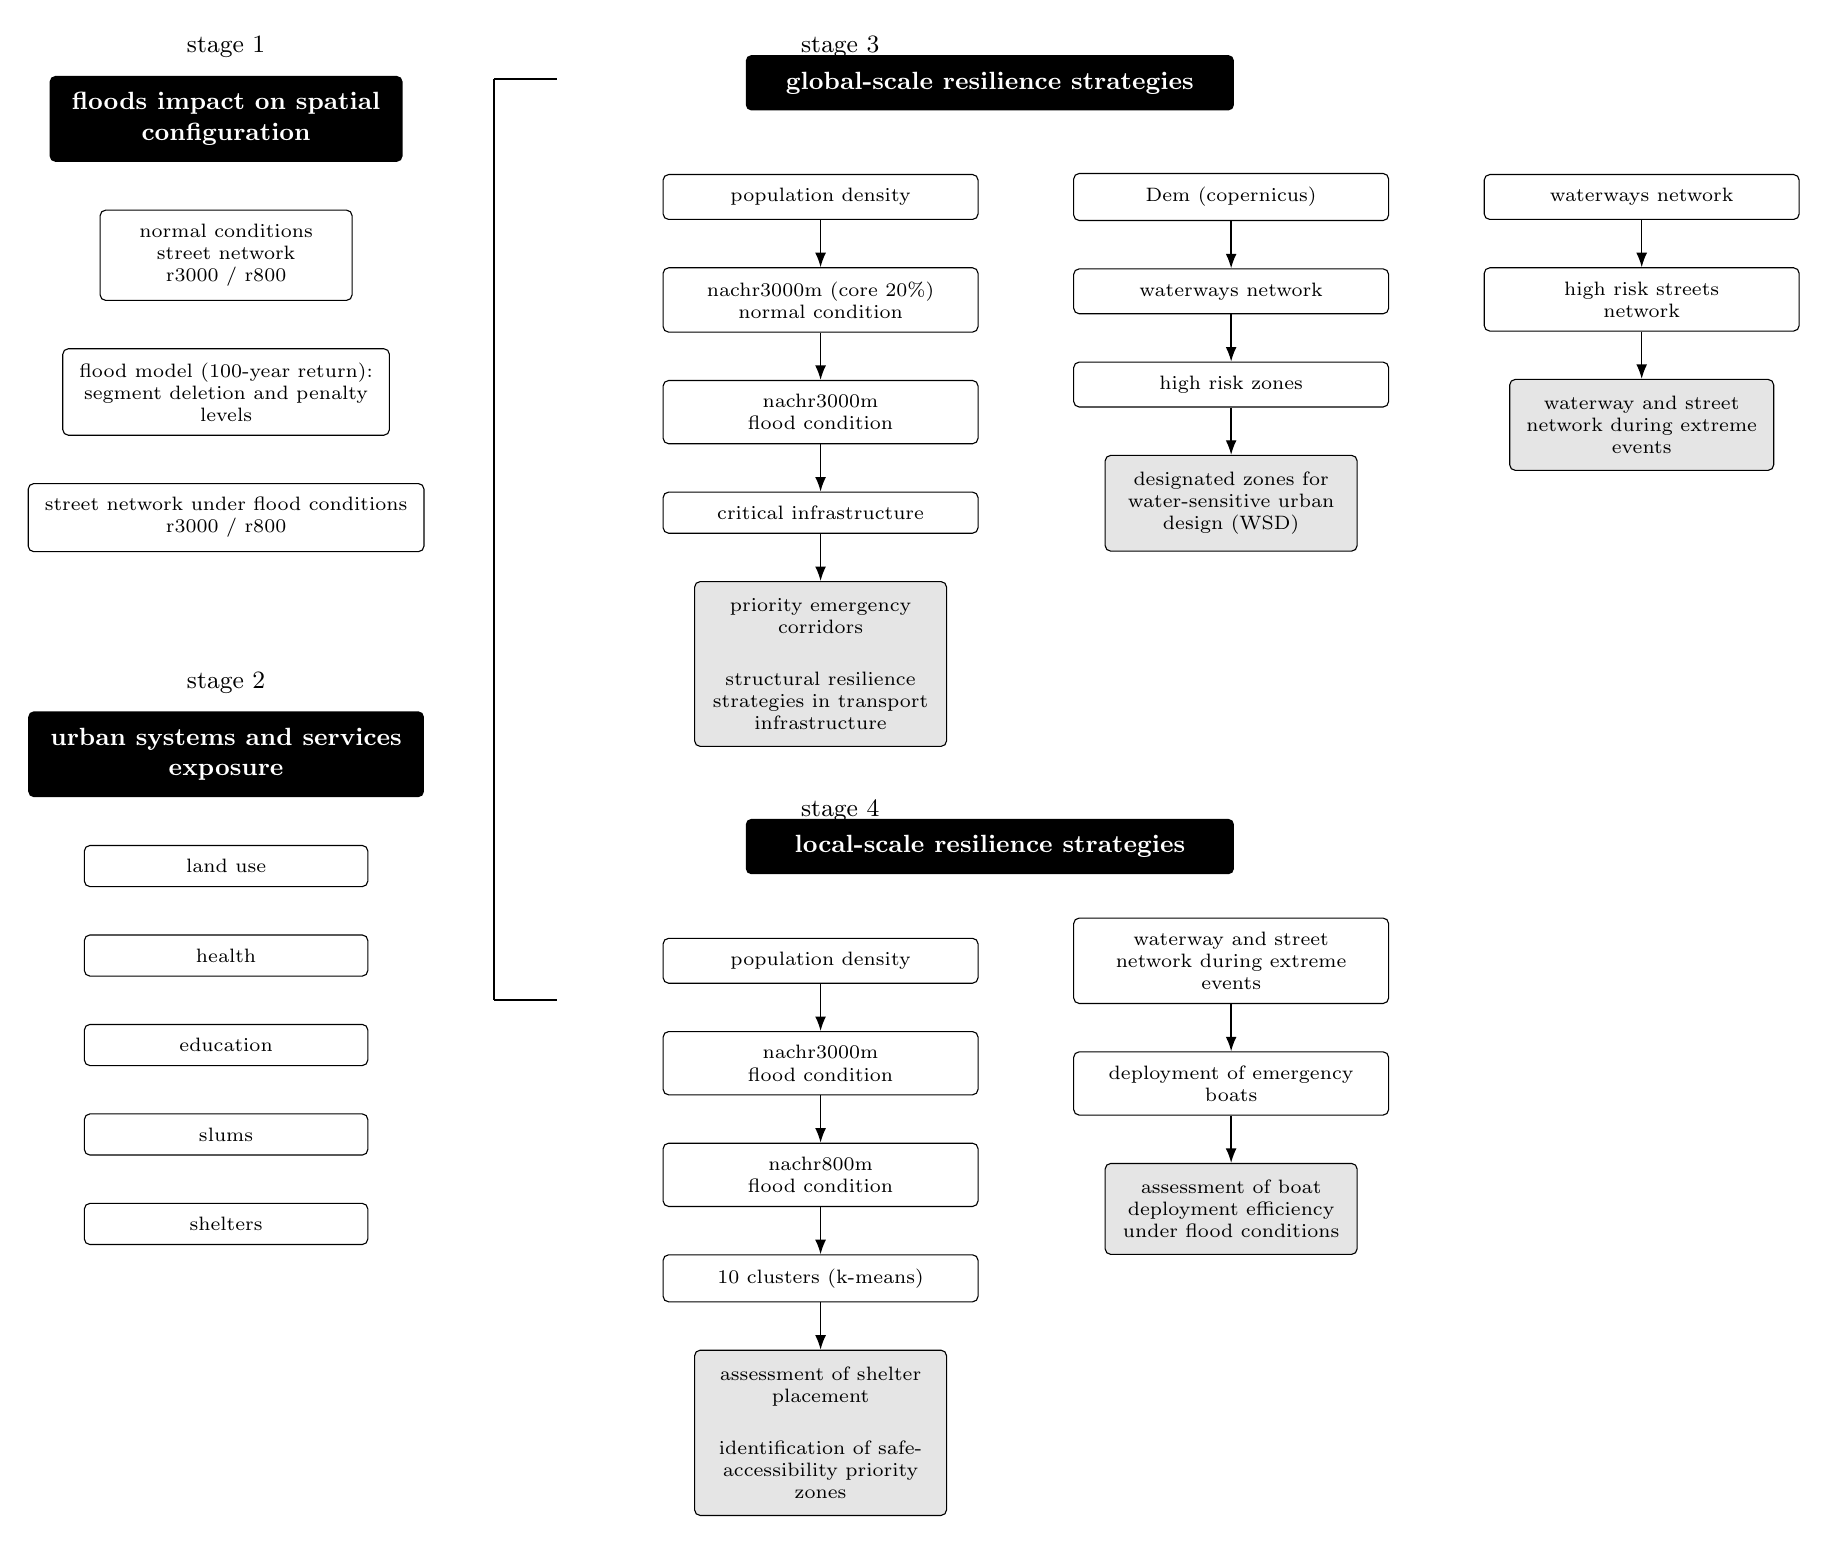
\begin{tikzpicture}[
  font=\fontfamily{phv}\selectfont,
  >=Latex,
  node distance=6mm and 10mm,
  stageLabel/.style={font=\small, align=left},
  bar/.style={fill=black, rounded corners=2pt, text=white, font=\small\bfseries, inner xsep=8pt, inner ysep=6pt, minimum width=6.2cm, align=center},
  box/.style={draw, rounded corners=2pt, fill=white, font=\scriptsize, inner xsep=6pt, inner ysep=5pt, align=center, minimum width=3.2cm},
  boxWide/.style={box, minimum width=4.0cm},
  outbox/.style={draw, rounded corners=2pt, fill=gray!20, font=\scriptsize\bfseries, inner xsep=6pt, inner ysep=6pt, align=center, minimum width=4.0cm},
  outSmall/.style={outbox, font=\scriptsize, minimum width=3.2cm},
  arrow/.style={-Latex, line width=0.5pt},
]

% --- Left column (Stages 1–2) ---
\node[stageLabel] (s1lbl) at (0, 3.5) {stage 1};
\node[bar, below=1mm of s1lbl, minimum width=3.6cm] (s1bar) {floods impact on spatial\\configuration};
\node[box, below=of s1bar] (s1a) {normal conditions\\street network\\r3000 / r800};
\node[box, below=of s1a] (s1b) {flood model (100-year return):\\segment deletion and penalty\\levels};
\node[box, below=of s1b] (s1c) {street network under flood conditions\\r3000 / r800};

\node[stageLabel, below=14mm of s1c] (s2lbl) {stage 2};
\node[bar, below=1mm of s2lbl, minimum width=3.6cm] (s2bar) {urban systems and services\\exposure};
\node[box, below=of s2bar, minimum width=3.6cm] (s2a) {land use};
\node[box, below=of s2a, minimum width=3.6cm] (s2b) {health};
\node[box, below=of s2b, minimum width=3.6cm] (s2c) {education};
\node[box, below=of s2c, minimum width=3.6cm] (s2d) {slums};
\node[box, below=of s2d, minimum width=3.6cm] (s2e) {shelters};

% --- Right column (Stages 3–4) ---
\begin{scope}[xshift=7.8cm]
  \node[stageLabel] (s3lbl) at (0, 3.5) {stage 3};
  \node[bar] (s3bar) at (1.9, 3.05) {global-scale resilience strategies};

  % Stage 3 left stack
  \node[boxWide, below=8mm of s3bar, xshift=-2.15cm] (g1a) {population density};
  \node[boxWide, below=of g1a] (g1b) {nachr3000m (core 20\%)\\normal condition};
  \node[boxWide, below=of g1b] (g1c) {nachr3000m\\flood condition};
  \node[boxWide, below=of g1c] (g1d) {critical infrastructure};
  \node[outSmall, below=of g1d] (g1o) {priority emergency\\corridors\\\vspace{1mm}\\structural resilience\\strategies in transport\\infrastructure};

  % Stage 3 middle stack
  \node[boxWide, right=12mm of g1a] (g2a) {Dem (copernicus)};
  \node[boxWide, below=of g2a] (g2b) {waterways network};
  \node[boxWide, below=of g2b] (g2c) {high risk zones};
  \node[outSmall, below=of g2c] (g2o) {designated zones for\\water-sensitive urban\\design (WSD)};

  % Stage 3 right stack
  \node[boxWide, right=12mm of g2a] (g3a) {waterways network};
  \node[boxWide, below=of g3a] (g3b) {high risk streets\\network};
  \node[outSmall, below=of g3b] (g3o) {waterway and street\\network during extreme\\events};

  % connectors stage 3
  \draw[arrow] (g1a) -- (g1b);
  \draw[arrow] (g1b) -- (g1c);
  \draw[arrow] (g1c) -- (g1d);
  \draw[arrow] (g1d) -- (g1o);

  \draw[arrow] (g2a) -- (g2b);
  \draw[arrow] (g2b) -- (g2c);
  \draw[arrow] (g2c) -- (g2o);

  \draw[arrow] (g3a) -- (g3b);
  \draw[arrow] (g3b) -- (g3o);

  % Stage 4 (placed well below Stage 3 to avoid overlaps)
  \node[stageLabel] (s4lbl) at (0, -6.2) {stage 4};
  \node[bar] (s4bar) at (1.9, -6.65) {local-scale resilience strategies};

  \node[boxWide, below=8mm of s4bar, xshift=-2.15cm] (l1a) {population density};
  \node[boxWide, below=of l1a] (l1b) {nachr3000m\\flood condition};
  \node[boxWide, below=of l1b] (l1c) {nachr800m\\flood condition};
  \node[boxWide, below=of l1c] (l1d) {10 clusters (k-means)};
  \node[outSmall, below=of l1d] (l1o) {assessment of shelter\\placement\\\vspace{1mm}\\identification of safe-\\accessibility priority\\zones};

  \node[boxWide, right=12mm of l1a] (l2a) {waterway and street\\network during extreme\\events};
  \node[boxWide, below=of l2a] (l2b) {deployment of emergency\\boats};
  \node[outSmall, below=of l2b] (l2o) {assessment of boat\\deployment efficiency\\under flood conditions};

  \draw[arrow] (l1a) -- (l1b);
  \draw[arrow] (l1b) -- (l1c);
  \draw[arrow] (l1c) -- (l1d);
  \draw[arrow] (l1d) -- (l1o);

  \draw[arrow] (l2a) -- (l2b);
  \draw[arrow] (l2b) -- (l2o);
\end{scope}

% --- Decorative bracket between left and right blocks ---
\draw[line width=0.7pt] (3.4, 3.1) -- (3.4, -8.6);
\draw[line width=0.7pt] (3.4, 3.1) .. controls (3.8, 3.1) and (3.9, 3.1) .. (4.2, 3.1);
\draw[line width=0.7pt] (3.4, -8.6) .. controls (3.8, -8.6) and (3.9, -8.6) .. (4.2, -8.6);

\end{tikzpicture}

  \caption{Methodological framework for flood-accessibility modelling.}
\end{figure}

Understanding the interaction between floods and urban spatial configuration is critical to developing resilient cities under increasing climate threats. This study focuses on the territory of Chennai and employs a multi-scalar, systemic approach to model the impacts of extreme flood events on urban networks. It proposes targeted resilience strategies at both global and local levels (Figure 2). To assess the reshaping of spatial structures under flood conditions, street network accessibility is contrasted in normal and flood scenarios. Two scales are considered: a broader accessibility radius (r3000) and a localized radius (r800). The normal network is evaluated against a 100-year return period flood model (OpenCity Data), generating penalty classifications: high (segments removed), moderate (75\% penalty), and low (25\% penalty). Flood overlays on the street network allow quantification of accessibility degradation and spatial disruptions caused by floodwaters. The reconfigured network is analysed to identify cascading effects on critical urban systems. Accessibility is evaluated across five domains: land use, health services, education infrastructure, informal settlements (slums), and emergency shelters \\citep{gcc2024}. Severity is categorized using a four-tier scale, ranging from high to null, based on the 100-year flood model. This enables spatial prioritization of interventions and reveals patterns of vulnerability. Resilience strategies are structured at both global and local scales. At the global level, population density, critical infrastructure, and baseline accessibility (top 20\% of NACHr3000) form the foundational layers. Flood-adjusted accessibility (NACHr3000) is analysed to identify key street and bridge segments requiring intervention. Emergency response routes are delineated by merging NACHr3000 under normal and flood conditions. These routes inform resilience measures using the Climate App (DELTARES platform). A Digital Elevation Model (Copernicus GLO-30 DEM) and waterway data (India Water Resources System) support identification of flood-prone zones. These are integrated with street network data to guide the application of water-sensitive design strategies. A complementary model combining water networks and flood-impacted accessibility is developed to support evaluations under extreme conditions. Although created for local analysis, this model remains available for future applications, including hybrid mobility strategies. At the local level, population density, flood-adjusted accessibility (NAINr800 and NAINr3000), and Google's Open Buildings dataset are aggregated at the block level. All data is normalized between 0 and 1 to ensure comparability. The clustering model is applied only in zones free from flooding, with the goal of identifying the safest areas. K-means clustering (k=10) prioritizes population density, followed by global and local accessibility. This enables localized strategic planning. Clustering results support evaluation of shelter locations (Disaster Risk Reduction Plan, GCC). Analysis confirms which emergency shelters maintain accessibility under flood conditions. Priority blocks are identified for future shelter allocation based on combined network and risk modeling. Based on the global waterways and impacted network model, a local-scale assessment of emergency boat placement (GCC) is conducted. The model evaluates their spatial alignment with local accessibility during flood events and identifies opportunities to enhance hybrid evacuation systems. The model remains adaptable for future mobility planning. This methodology culminates in an integrated framework that links normal and flood-condition accessibility with socio-infrastructural vulnerabilities. By combining global-scale interventions--- such as route prioritization---with localized analyses of shelter and boat-based accessibility, the framework delivers a comprehensive resilience strategy. It balances immediate emergency needs with long-term adaptive planning and offers a scalable model for cities confronting hydro-climatic disruption.


\section{Results and Analysis}
Flood scenarios produced pronounced disruptions in Chennai's urban accessibility structure. The comparison of street networks under normal (NAINr3000, NACHr3000) and flood conditions (NAINr3000, NACHr3000 flood scenario) revealed a systemic reduction in accessibility. Street segments decreased by 6.56\% post-flood impact. Global accessibility indices dropped significantly: NAINr3000 by 19.74\% and NACHr3000 by 18.10\% (Figure 3). In finer-grained, local analyses (r800 radius), accessibility fell by 15.23\% for NAINr800 and by 3.14\% for NACHr800 (Figure 4). These reductions highlight the spatial fragility of Chennai's urban fabric under extreme hydrological events (Table 1).

\begin{figure}[ht]
  \centering
  \includegraphics[width=\textwidth,page=2]{../../figures/chennai_maps.pdf}
  \caption{Global and local accessibility under normal and flood conditions (source atlas: \texttt{figures/chennai\_maps.pdf}).}
\end{figure}

\begin{table}[ht]
  \centering
  \caption{Mean values of accessibility indicators and network segments under normal and flood conditions.}
  \begin{tabular}{lrrr}
    \toprule
    Metric & Normal & Flood & Difference \\
    \midrule
    Segments & -- & -- & -6.56\% \\
    NAIN r3000 & 0.8217 & 0.6595 & -19.74\% \\
    NACH r3000 & 0.8110 & 0.6642 & -18.10\% \\
    NAIN r800 & 0.9219 & 0.7815 & -15.23\% \\
    NACH r800 & 0.8458 & 0.8192 & -3.14\% \\
    \bottomrule
  \end{tabular}
\end{table}

Accessibility loss manifested heterogeneously across critical urban functions, with marked differences among urban fragments. High-risk areas accounted for a significant proportion of degraded accessibility: 35 health infrastructure units, 72 educational facilities, 163 slums, and 45 shelters were in high-risk zones. Health services and slums exhibited the highest concentration in these high-risk fragments, reflecting acute vulnerabilities during extreme flood events. Educational facilities also faced considerable exposure, with a notable number situated in zones with high penalty accessibility loss. Conversely, most shelters were distributed in fragments categorized as null or moderate risk, yet a non-negligible portion remained exposed within highrisk areas. These findings underline systemic misalignments between critical services and resilient urban structures, leaving essential infrastructure and marginalized communities especially vulnerable during flood events. The analysis of urban land use across different fragments revealed that residential areas accounted for the largest share of flood-affected zones, particularly in the highly impacted categories. Agricultural and open space areas demonstrated lower exposure, while commercial and institutional zones were moderately impacted. Fragments with a predominance of residential and mixed-residential land uses displayed the greatest decline in accessibility (Figure 5). This spatial configuration underscores the vulnerability of densely populated and economically vital areas, emphasizing the urgent need for targeted resilience strategies in these land use categories. Detailed evaluation from Table 2 shows differentiated impacts across city fragments. In Fragment 1, critical infrastructures such as health and educational services, slums, and shelters concentrated significantly in high-risk zones, with health units and slums showing the most acute vulnerability. Fragment 2 exhibited a comparatively moderate distribution, while Fragment 3, though smaller in size, demonstrated a disproportionately high exposure of slums and shelters to flood risk. Fragment 4 presented the highest number of affected slums and shelters across all categories, indicating extreme vulnerability. Fragment 5, despite its smaller representation, continued the pattern of infrastructure exposure to high-risk areas. This fragment-by-fragment breakdown highlights the heterogeneity of urban vulnerability and supports the design of localized, fragment-specific resilience interventions.

number of blocks

level of risk per fragment

Figure 5. Critical infrastructure overlaid with flood level of risk in the five- fragments. The map highlights the distribution of services (health, education, slums, shelters) in relation to spatial risk categories across Chennai's five urban fragments.

level of risk per fragment

number of infraestructure or services

Table 2. Overlay of infrastructure or services and accessibility class by urban fragment.

Global-Scale Strategies: Emergency Routes and Critical Zone Identification The top 20\% of highly accessible routes (NACHr3000 under normal conditions) served as the backbone for modelling emergency priority networks. Integrating these routes with the floodconditioned accessibility model enabled the identification of strategic corridors essential for evacuation and supply continuity. The emergency response network specifically ensured the connection of Chennai's most critical infrastructures, including the main hospitals, the airport, and the port, as well as the densest urban areas. Emergency response routes, limited to the main connections network, were proposed as a strategic guide to optimize the allocation of emergency resources during flood events. Specific interventions were tailored according to infrastructure type: for streets, strategies included gutter inclination adjustments, the elevation of evacuation pathways, and the reinforcement of Water-Sensitive Design principles; for bridges, interventions emphasized structural reinforcement, elevation to mitigate flood impacts, and ensuring redundancy in case of partial network failure. These proposals aim to enhance the functionality of the principal mobility corridors under extreme conditions (see Figure 6).

\begin{figure}[ht]
  \centering
  \includegraphics[width=\textwidth,page=6]{../../figures/chennai_maps.pdf}
  \caption{Priority corridors and city-wide intervention areas under flood conditions (source atlas: \texttt{figures/chennai\_maps.pdf}).}
\end{figure}

Leveraging a Digital Elevation Model (Copernicus GLO-30), which served to identify the city's lowest-lying areas, combined with waterways and water bodies data from the India Water 

Resources Information System, a comprehensive floodplain analysis was conducted. The identified low-lying zones were cross-referenced with high flood-risk areas, showing strong spatial coincidence. Based on this overlap, zones suitable for floodplain excavation were proposed, prioritizing large open spaces identified through recent satellite imagery. Furthermore, areas where residential buildings were detected using Google's Open Buildings dataset were flagged for density management or growth restriction strategies, aiming to mitigate future flood vulnerability through adaptive urban planning. This multi-layered model provided the foundation for a robust global-scale resilience strategy, balancing immediate flood responses with long-term urban planning interventions (see figure 7).

Figure 7. Proposed floodplain intervention zones based on elevation and hydrological data.

At a local scale (NAINr800 and NACHr800), a complementary waterways and flood-impacted street network model was developed, offering a foundation for hybrid land-water mobility strategies. Although primarily designed to evaluate accessibility during floods, this model remains available for future expansion into integrated resilience frameworks. Local-Scale Strategies: Safe Zones and Shelter Accessibility The waterways and flood street network model were utilized to assess the accessibility of existing emergency boat deployment points managed by the Greater Chennai Corporation (see figure 8). 

Analysis revealed that 30.38\% of boat locations were within highly accessible zones (NAINr800 > 1.0), while 31.65\% were positioned in areas of lowest accessibility (NAINr800 $\leq$ 0.6). A more detailed histogram breakdown showed that 8.86\% of boats were in zones of excellent accessibility (NAINr800 > 1.2), 21.52\% in high-accessibility zones (1.0 < NAINr800 $\leq$ 1.2), and 22.78\% in moderately accessible areas (0.8 < NAINr800 $\leq$ 1.0), reinforcing the uneven distribution of resources across accessibility gradients (figure 9 and table 3). This distribution highlights critical vulnerabilities, particularly for peripheral and flood-prone neighbourhoods, underscoring the need for strategic relocation or augmentation of boat deployment points. This uneven distribution of emergency boat resources suggests critical gaps in flood-time accessibility, especially in peripheral and low-lying neighbourhoods. The model highlights strategic locations where new or relocated boat points could enhance flood resilience, supporting the development of hybrid land-water evacuation networks. Although primarily serving to evaluate current operational capacities, the accessibility model also establishes a baseline for future resilience strategies, enabling Chennai to incorporate waterbased mobility into its urban adaptation planning.

Figure 8. Distribution of emergency boats under flood conditions.

The figure shows the location of deployed emergency boats in relation to floodadjusted accessibility (r800), highlighting spatial disparities in coverage across safe and vulnerable zones.

Figure 9. Accessibility histogram of emergency boat locations (NAINr800)

Measures NAINr800m

boats

(\%)

NAINr800m > 1.2

8.86\%

1.0 < NAINr800m $\leq$ 1.2

21.52\%

0.8 < NAINr800m $\leq$ 1.0

22.78\%

0.6 < NAINr800m $\leq$ 0.8

15.19\%

NAINr800m $\leq$ 0.6

31.65\%

Table 3. Distribution of emergency boat locations (NAINr800)

A k-means clustering analysis based on normalized population density, global accessibility (NAINr3000), and local accessibility (NAINr800) revealed ten distinct safe clusters within the norisk zones (see Figure 10). Clusters 7 and 9 emerged as the most strategically important safe zones. Cluster 7, while comprising only 90 blocks, displayed a highly concentrated and cohesive distribution pattern, predominantly located within specific city sectors, making it ideal for focused and immediate intervention strategies. Cluster 9, by contrast, included 50,424 blocks, with a broad geographic distribution across the city's five main urban fragments. Its dispersion allows for a widespread coverage of resilience actions, ensuring accessibility to a wider population base. Additionally, Cluster 9 exhibited consistently high normalized population density (0.43906) and accessibility (NAINr800 of 0.41081 and NAINr3000 of 0.33262), supporting its designation as a critical backbone for local-scale resilience strategies (see table 4 and 5). This detailed assessment confirms that Clusters 7 and 9 provide complementary opportunities: one for concentrated resource allocation and the other for widespread territorial resilience planning, making them priority candidates for safe zone designation and strategic emergency planning.

\begin{figure}[ht]
  \centering
  \includegraphics[width=\textwidth,page=4]{../../figures/chennai_maps.pdf}
  \caption{Population density, accessibility, and safe zones under normal and flood conditions (source atlas: \texttt{figures/chennai\_maps.pdf}).}
\end{figure}

Shelter evaluation indicated that a substantial portion of existing emergency shelters were not optimally located (see Figure 11). Detailed analysis using the Range-Shelters table revealed that only 41 shelters (22.4\% of the total) were located within the optimal 100--400-meter distance from highly accessible areas. A smaller number, 14 shelters (7.6\%), were situated within 50-100 meters, and just 8 shelters (4.4\%) were positioned within the ideal proximity of 10-50 meters. Alarmingly, 89 shelters (48.6\%) were located over 400 meters away, significantly reducing their effective accessibility during flood emergencies (see table 6). This misalignment highlights critical gaps in current emergency infrastructure planning and signals the need for a strategic reassessment of shelter locations to ensure timely and equitable access for the most vulnerable populations during extreme events.

\begin{figure}[ht]
  \centering
  \includegraphics[width=0.8\textwidth,page=5]{../../figures/chennai_maps.pdf}
  \caption{Shelter evaluation and accessibility under flood conditions (source atlas: \texttt{figures/chennai\_maps.pdf}).}
\end{figure}

Cluster

Normalized\_Population Density

0.16478

0.34052

0.23625

0.30099

0.69862

0.22445

0.49269

0.42266

0.43906

0.48422

Normalized\_NAINr800

0.29464

0.28554

0.40100

0.91973

0.26662

0.20296

0.61516

0.20180

0.41081

0.29869

Normalized\_NAINr3000

0.24595

0.25831

0.31962

0.92057

0.23364

0.18593

0.60203

0.18714

0.33262

0.26100

Table 4. Results of k-mean process with normalized values of population and NAIN identifies Zones 7 and 9 as high-priority safe zones for flood preparedness and local intervention. Number of blocks in each cluster

76956.000

128831.000

41142.000

5.000

48681.000

70231.000

90.000

93296.000

50424.000

96273.000

Cluster

Table 5. Number of blocks in each cluster

Figure. 11. Distribution of emergency shelters under flood conditions. Range >401 m 100-400 m 50-100 m 10-50 m 0-10 m

Shelters

Table 6. Shelter distribution by walking distance under flood conditions (NAINr800)

The results consolidate into a comprehensive, multi-scalar resilience framework. At the global scale, critical corridors, floodplain interventions, and emergency routes were identified to safeguard urban systems under extreme events. Locally, clustering analysis pinpointed safe zones for emergency shelter prioritization, while boat accessibility evaluations highlighted urgent areas for mobility reinforcement. This integrated approach not only addresses immediate hydrological threats but also lays the groundwork for a future-proof urban system, capable of absorbing, adapting, and responding to intensifying hydro-climatic pressures. The methodologies and findings present a replicable, scalable model for other flood-vulnerable cities navigating the complexities of urban resilience in the 21st century.


\section{Discussion}
The findings of this study underscore the role of urban spatial configuration in modulating Chennai's resilience to extreme flood events. Accessibility losses across different radii (r3000 and r800) confirm that not only the physical extent of floods but also the systemic organization of the street network critically shape impacts. Broad-scale accessibility (NAINr3000) experienced significant decline under flooding, while localized accessibility (NACHr800) retained partial functionality, highlighting differentiated vulnerabilities across scales. Compact urban forms, such as Cluster 7, displayed resilience by concentrating accessibility, while the broader dispersion of Cluster 9 emphasized the importance of redundancy across the urban system. The strategic design of emergency priority routes ensured the accessibility of key infrastructures, such as hospitals, the airport, and the port. Focusing on the top 20\% of accessible corridors under flood scenarios illustrates that selective infrastructural reinforcement can preserve critical urban functionality. Moreover, analysing emergency boat deployment zones introduced the need for hybrid mobility systems. The uneven distribution of boats in Chennai highlights critical gaps in flood-time accessibility, reinforcing that diversified evacuation options---across land and water--- are vital to urban resilience. Cross-referencing elevation, flood risk, land use, and infrastructure data revealed strong spatial coincidence between environmental vulnerability and socio-economic density. Nature-based interventions, such as floodplain excavations and density management strategies, emerge as essential for mitigating risk. Integrating spatial and environmental logics advances WaterSensitive Urban Design (WSUD) principles, ensuring interventions align with natural hydrological patterns. Restoring Chennai's historic relationship with its waterways and floodplains is critical to reducing systemic flood risk and reestablishing the city's natural capacity for resilience. The analysis confirms that Chennai's exposure to floods stems from deep-seated structural vulnerabilities: rapid demographic growth, governance deficiencies, data scarcity, and environmental degradation. These findings align with Lavell's (2003) argument that disasters are not natural, but the result of accumulated socio-spatial vulnerabilities embedded within territorial and urban systems. Recognizing disasters as socially constructed reframes resilience from a reactive posture toward proactive, structural urban adaptation, addressing the root causes rather than merely the symptoms of vulnerability. 

Several limitations must be acknowledged. The accessibility analysis relies on static flood modelling based on a 100-year return period, whereas dynamic, multi-scenario modelling could capture temporal variability more accurately. Additionally, although this study integrates population density and land use, detailed demographic vulnerability metrics (such as age, disability, or income) could not be fully incorporated due to data limitations, notably following Chennai's administrative restructuring from 150 to 200 wards post-2011. Future research could enhance this model by incorporating social vulnerability indices and simulating real-time accessibility shifts under flood conditions. Hybrid mobility systems could also be expanded by exploring autonomous watercraft and amphibious evacuation strategies. This study advances a multi-scalar, interdisciplinary framework that synthesizes spatial configuration analysis with environmental vulnerability assessments to guide urban resilience strategies. Prioritizing accessibility reinforcement, integrating nature-based interventions, and recognizing the structural nature of urban risks offer a replicable model for cities in the Global South confronting intensifying hydro-climatic threats. By highlighting systemic vulnerabilities and proposing hybrid resilience solutions, this work contributes to building cities that not only survive but adapt to future extremes.


\section{Conclusions}
This paper demonstrates a transferable workflow to quantify accessibility loss under flood disruption and to derive priority intervention corridors.

Future work can extend the approach with scenario ensembles, sensitivity tests on disruption thresholds, and validation against observed service outages and travel constraints during flood events.


\section{References}
\nocite{*}
\bibliographystyle{apalike}
\bibliography{references}

\end{document}
